\documentclass[10pt,a4paper]{article}
\usepackage[utf8]{inputenc}
\usepackage{amsmath}
\usepackage{amsfonts}
\usepackage{amssymb}
\usepackage{makeidx}
\usepackage{graphicx}
\usepackage[left=2cm,right=2cm,top=2cm,bottom=2cm]{geometry}
\author{Jiménez Cortés Raúl}

\begin{document}
\begin{center}
\begin{LARGE}
\textbf{INGENIERÍA MECATRÓNICA}\\
\end{LARGE}
{\large Sistemas Eletrónicos De Interfaz}\\
\begin{figure}[hbtp]
\centering

\includegraphics[scale=0.80]{UPZMG_Mecatr_nica.png}
\end{figure} 
\begin{center}
\begin{LARGE}
EV-2-4-Giro De Un Motor De Corriente Directa.
\end{LARGE}
\end{center}

\begin{Large}
\textbf{Alumno}
\\\textit{Raúl Jiménez Cortés}
\textbf{\\Maestro}
\\\textit{Morán Garabito Carlos Enriquez}
\textbf{\\Fecha de Entrega}
\\\textit{15/10/2019}
\textbf{\\Grupo}
\\\textit{4º "B"}
\end{Large}
\end{center}

\newpage
\section{Motor De Corriente Directa}
Los motores de Corriente Directa o motor DC(correspondiente a las iniciales en inglés “direct current”) es también conocidos como motor de Corriente Continua o motor CC, son  muy utilizados en diseños de ingeniería debido a las características torque-velocidad que poseen con diferentes configuraciones eléctricas o mecánicas.
Motor de corriente directa.

Una gran ventaja de los motores de CD se debe a que es posible controlarlos con suavidad y en la mayoría de los casos son reversibles, responden rápidamente gracias a que cuentan con una gran razón de torque a la inercia del rotor. Otra ventaja es la implementación del frenado dinámico, donde la energía generada por el motor se alimenta a un resistor disipador, y el frenado regenerativo donde la energía generada por el motor retroalimenta al suministro de potencia CD, esto es muy utilizado en aplicaciones donde se deseen frenados rápidos y de gran eficiencia.

\begin{center}
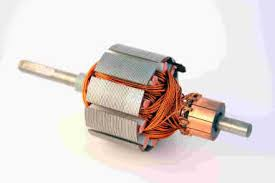
\includegraphics[scale=0.5]{1.png} 
\end{center}

\section{Clasificación de los Motores de CD}
Los motores de corriente directa se pueden clasificar de acuerdo con la forma en que crean los campos magnéticos del estator.\\
-Imán permanente\\
-Devanado shunt\\
-Devanado serie\\
-Devanado compuesto\\
\textbf{Curva Torque - Velocidad}
La siguiente gráfica es una representación de los torques que un motor puede proporcionar a diferentes velocidades a los voltajes nominales.\\

\begin{center}
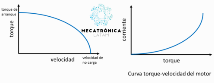
\includegraphics[scale=0.5]{2.png} 
\end{center}

Para un dado torque proporcionado por el motor, se puede utilizar la curva corriente-torque para determinar la corriente requerida cuando se le aplica el voltaje nominal al motor.  

Como regla general, los motores generan grandes torques a baja velocidad, y grandes torques implican una demanda mayor de corriente por parte del motor.

El torque de arranque o torque crítico (Ts): Es el torque máximo que puede proporcionar un motor a velocidad cero, asociado con el arranque o sobrecarga del motor.

La velocidad de no carga Wmáx: Es la máxima velocidad sostenida que puede lograr el motor. Esta velocidad sólo se puede lograr cuando no se aplica carga o torque al motor.\\
\textbf{Motores de Imán Permanente (PM)}
En este tipo de motores, los campos del estator son generados mediante imanes permanentes que no requieren fuente de alimentación externa y por lo tanto no producen un calentamiento. Los motores PM son más ligeros y pequeños en comparación con otros motores de CD con algunas características equivalentes ya que la intensidad del campo del imán permanente es alta. También resulta sencillo invertir el sentido de giro al conmutar la dirección del voltaje aplicado, ya que la corriente y el campo cambian de dirección sólo en el rotor.

El motor de imán permanente es ideal en aplicaciones de control por computadora debido a su linealidad torque-velocidad, aunque únicamente se utilizan en aplicaciones de baja potencia pues su potencia nominal usualmente se limita a 5 hp (3278 W) o menos.

Los motores CD de imán permanente pueden ser motores con escobillas, sin escobillas o de pasos.\\

\begin{center}
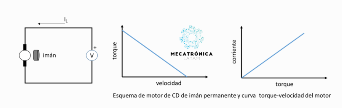
\includegraphics[scale=0.5]{3.png} 
\end{center}

\textbf{Motor Shunt}
Conformados por una armadura y devanados de campo conectados en paralelo que son activados mediante la misma fuente. Los motores shunt presentan velocidad casi constante sobre un gran rango de carga, cuentan con un torque de arranque de aproximadamente 1.5 veces el torque operativo nominal, tienen torque de arranque más bajo que cualquiera de los motores de CD y se puede convertir económicamente para permitir una velocidad ajustable al colocar un potenciómetro en serie con los devanados de campo. La corriente de carga total es la suma de las corrientes de armadura y campo.\\

\begin{center}
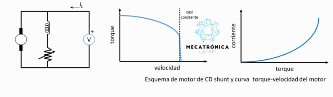
\includegraphics[scale=0.5]{4.png} 
\end{center}

\textbf{Motor Serie}
Cuentan con devanados de armadura y campo conectados en serie, de modo que las corrientes de armadura y campo son iguales. Los motores en serie generan torques de arranque muy altos, velocidad extremadamente variable dependiendo de la carga, y gran velocidad cuando la carga es pequeña.

Los motores en serie grandes pueden fallar catastróficamente cuando se descargan súbitamente debido a la fuerza dinámica a altas velocidades, a esto se le llama sin control.  

La curva torque-velocidad para un motor en serie tiene forma hiperbólica, lo que implica una relación inversa entre el torque y la velocidad, con una potencia casi constante.\\

\begin{center}
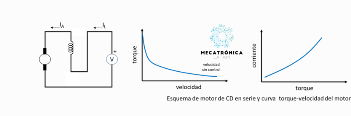
\includegraphics[scale=0.5]{5.png} 
\end{center}

\textbf{Motor Compuesto}
Estos motores incluyen tanto devanados de campo en derivación como en serie, lo que resulta en características combinadas de motores en derivación y en serie.

Parte de la corriente de carga pasa a través de los devanados de armadura y serie, la corriente de carga restante pasa sólo a través de los devanados en derivación. La velocidad máxima de un motor compuesto es limitada, su regulación de velocidad no es tan buena como la de un motor en derivación. El torque producido por los motores compuestos es un poco menor que el de los motores en serie de similar tamaño.\\

\begin{center}
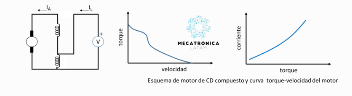
\includegraphics[scale=0.5]{6.png} 
\end{center}

\textbf{PARTES QUE INTEGRAN UN MOTOR COMÚN DE CORRIENTE DIRECTA}

\begin{center}
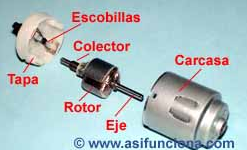
\includegraphics[scale=0.5]{7.png} 
\end{center}

Un motor común de corriente directa o continua se compone de las siguientes partes o piezas:\\

\begin{center}
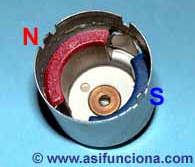
\includegraphics[scale=0.5]{8.png} 
\end{center}

• Carcasa metálica o cuerpo del motor. Aloja en su interior, de forma fija, dos imanes permanentes con forma de semicírculo, con sus correspondientes polos norte y sur.


• Rotor o parte giratoria del motor. Se compone de una estructura metálica formada por un conjunto de chapas o láminas de acero al silicio, troqueladas con forma circular y montadas en un mismo eje con sus correspondientes bobinas de alambre de cobre, que lo convierten en un electroimán giratorio. Por norma general el rotor de la mayoría de los pequeños motores de C.D. se compone de tres enrollados o bobinas que crean tres polos magnéticos. Los extremos de cada una de esas bobinas se encuentran conectados a diferentes segmentos del colector.

• Colector o conmutador. Situado en uno de los extremos del eje del rotor, se compone de un anillo deslizante seccionado en dos o más segmentos. Generalmente el colector de los pequeños motores comunes de C.D. se divide en tres segmentos.

• Escobillas. Representan dos contactos que pueden ser metálicos en unos casos, o compuesto por dos piezas de carbón en otros. Las escobillas constituyen contactos eléctricos que se deslizan por encima de los segmentos del colector mientras estos giran. Su misión es suministrar a la bobina o bobinas del rotor a través del colector, la corriente eléctrica directa necesaria para energizar el electroimán. En los pequeños motores las escobillas normalmente se componen de dos piezas o flejes metálicos que se encuentran fijos en la tapa que cierra la carcasa o cuerpo del motor.\\

\begin{center}
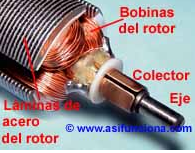
\includegraphics[scale=0.5]{9.png} 
\end{center}

• Tapa de la carcasa (izquierda en la foto). Es la tapa que se emplea para cerrar uno de los extremos del cuerpo o carcasa del motor. En su cara interna se encuentran situadas las escobillas de forma fija. El motor de esta foto utiliza en función de escobillas dos flejes metálicos.\\

\begin{center}
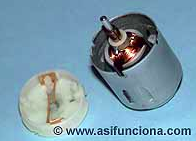
\includegraphics[scale=0.5]{10.png} 
\end{center}

\textbf{PRINCIPIO DE FUNCIONAMIENTO DEL MOTOR DE CORRIENTE DIRECTA}
El principio de funcionamiento de los motores eléctricos de corriente directa o continua se basa en la repulsión que ejercen los polos magnéticos de un imán permanente cuando, de acuerdo con la Ley de Lorentz, interactúan con los polos magnéticos de un electroimán que se encuentra montado en un eje. Este electroimán se denomina “rotor” y su eje le permite girar libremente entre los polos magnéticos norte y sur del imán permanente situado dentro de la carcasa o cuerpo del motor.

Cuando la corriente eléctrica circula por la bobina de este electroimán giratorio, el campo electromagnético que se genera interactúa con el campo magnético del imán permanente. Si los polos del imán permanente y del electroimán giratorio coinciden, se produce un rechazo y un torque magnético o par de fuerza que provoca que el rotor rompa la inercia y comience a girar sobre su eje en el mismo sentido de las manecillas del reloj en unos casos, o en sentido contrario, de acuerdo con la forma que se encuentre conectada al circuito la pila o la batería.


Función del colector o conmutador en el motor de C.D.

En la siguiente figura se representa, de forma esquemática y simplificada, la vista frontal de un colector seccionado en dos partes, perteneciente a un motor de corriente directa (C.D.) muy simple. También se muestra el enrollado de la bobina del electroimán que gira a modo de rotor, diferenciada por un color diferente en cada una de sus mitades. Una de las mitades se representa por un círculo rojo y la otra por un círculo azul, identificados como “1” y “2”. Como se puede ver, uno de los terminales de dicha bobina se encuentra conectado a la sección “a” del colector y el otro terminal a la sección “b”.\\

\begin{center}
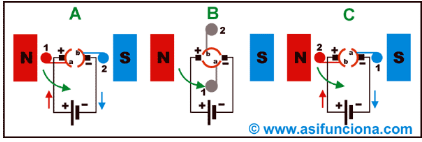
\includegraphics[scale=0.5]{11.png} 
\end{center}

En el motor de corriente directa el colector o conmutador sirve para conmutar o cambiar constantemente. el sentido de circulación de la corriente eléctrica a través del enrollado de la bobina del rotor  cada  vez. que completa media vuelta. De esa forma el polo norte del electroimán coincidirá siempre con el también. polo. norte del imán permanente y el polo sur con el polo sur del propio imán. Al coincidir siempre dos. polos magnéticos, que en todo momento van a ser iguales, se produce un rechazo constante entre. ambos, lo que permite al rotor mantenerse girando ininterrumpidamente sobre su eje durante. todo el. tiempo que se encuentre conectado a la corriente eléctrica.

Tal como vemos, en “A” de la figura, la bobina del electroimán se encuentra colocada entre los polos norte “N” y sur “S” del campo magnético del imán permanente. A su vez, el polo positivo (+) de la batería se encuentra conectado siguiendo el sentido convencional de la corriente (del signo positivo al negativo) en la mitad “a” del colector a través de la escobilla identificada también con el signo (+). De esa forma la mitad de la bobina de color rojo (1) se energiza positivamente para formar el polo norte “N”, mientras que la otra mitad, la de color azul (2) se energiza negativamente para formar el polo sur “S”.

Como resultado, cuando en el electroimán se forma el polo norte, de inmediato el también polo norte del imán permanente lo rechaza. Al mismo tiempo el polo sur que se forma en el extremo opuesto, es rechazado igualmente por el polo sur del propio imán; por tanto se produce una fuerza de repulsión en ambos extremos del rotor al enfrentarse y coincidir con dos polos iguales en el imán permanente. Si bajo esas condiciones aplicamos la “Regla de la mano izquierda” y tomamos como referencia, por ejemplo, la parte de la bobina donde se ha formado el polo norte en el electroimán, comprobaremos que al romper la inercia inicial, comenzará a girar en dirección contraria a las manecillas del reloj, como indica la flecha de color verde.

Una vez que la bobina del electroimán gira y asume una posición vertical (como se muestra en la parte “B” de la ilustración), las escobillas dejan de hacer contacto con ambos segmentos del colector. En esa posición neutra la corriente que suministra la batería deja de circular y la bobina se desenergiza, por lo que ambos extremos del electroimán pierden momentáneamente sus polos magnéticos. No obstante, debido a la fuerza de inercia o impulso de giro que mantiene el electroimán, esa posición la rebasa de inmediato y sus extremos pasan a ocupar la posición opuesta a la que tenían, tal como se muestra en la parte “C” de la misma ilustración.

Ahora en “C” se puede ver que la mitad de la bobina que anteriormente tenía color azul (2) con polaridad sur cuando se encontraba situada a la derecha del eje del rotor pasa a ocupar la parte izquierda junto con la mitad (b) del colector al que se encuentra conectada. Esa parte de la bobina que ha girado, al ocupar ahora la posición opuesta, se convierte en el polo norte (2) del electroimán por lo que es rechazado de nuevo por el polo norte del imán permanente, que como ya se explicó se encuentra fijo al cuerpo del motor. Seguidamente el electroimán, al continuar girando y dar otra media vuelta, pasa de nuevo por la zona neutra (como en “B”) repitiéndose de nuevo el mismo ciclo. Esos cambios continuos en los polos del electroimán del rotor que proporciona el colector, son los que permiten que se mantenga girando de forma ininterrumpida mientras se mantenga energizado.

En resumen, la función del colector es permitir el cambio constante de polaridad de la corriente en la bobina del electroimán del rotor para que sus polos cambien constantemente. Este cambio ocurre cada vez que el electroimán gira media vuelta y pasa por la zona neutra, momento en que sus polos cambian para que se pueda mantener el rechazo que proporciona el imán permanente. Esto permitirá que el electroimán del rotor se mantenga girando constantemente durante todo el tiempo que la batería o fuente de fuerza electromotriz (F.E.M.) se mantenga conectada al circuito del motor, suministrándole corriente eléctrica.\\

\begin{center}
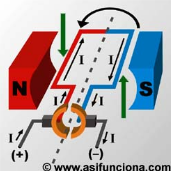
\includegraphics[scale=0.5]{12.png} 
\end{center}

 En esta otra ilustración se muestra, de forma esquemática y simplificada, un motor común de corriente directa (C.D.) con un rotor formado por una simple bobina de una sola espira de color rojo y azul, para diferenciar cada mitad. Si seguimos el recorrido de la corriente eléctrica (I) asumiendo que fluye en el sentido convencional (del polo positivo "+" al polo negativo "–" de la batería, según indican las flechas negras), cuando en la mitad izquierda de la espira de color rojo se forma el polo norte “N” coincidiendo con la misma polaridad del campo magnético del imán permanente fijo al cuerpo del motor, se produce una fuerza de rechazo entre ambos polos iguales. Si aplicamos la “Regla de la mano izquierda” se puede determinar que esa mitad de la espira se moverá hacia abajo (flecha verde izquierda). Por otra parte, en la mitad derecha (de color azul) ocurrirá lo mismo, pero a la inversa, por lo que aplicando la propia regla comprobaremos que se moverá hacia arriba (flecha verde derecha). 

La combinación de esas dos fuerzas o vectores actuando de forma opuesta y al unísono (de acuerdo con la Fuerza de Lorentz), provocará que el electroimán del rotor, formado aquí por esa simple espira, comience a girar en torno a su eje imaginario (representado por una línea de puntos en la figura) en dirección contraria a las manecillas de reloj en este ejemplo. Ese movimiento de rotación se encuentra señalado por la flecha negra en forma de semicírculo, que se encuentra dibujada al fondo de la espira.\\
\textbf{FUNCIONAMIENTO DE UN MOTOR COMÚN DE CORRIENTE DIRECTA}
La siguiente figura muestra, de forma animada, el funcionamiento de un motor común bipolar de corriente directa. Como se puede observar, éste consta de un imán permanente en forma de semicírculo, dividido en dos partes fijas al cuerpo del motor. La parte de color rojo del imán corresponde al polo norte “N” y la azul al polo sur “S”. También encontramos un electroimán que a modo de rotor gira entre los polos magnéticos del imán permanente. En el eje del rotor se muestra un colector dividido en dos segmentos y dos escobillas haciendo contacto con los mismos. La batería se encuentra conectada de tal forma que la corriente eléctrica fluye en el sentido convencional con el polo positivo (+) conectado a la escobilla derecha y el polo negativo (–) a la escobilla izquierda. Cada escobilla hace pleno contacto con las secciones del colector, incluso mientras el rotor se encuentra girando.

\begin{center}
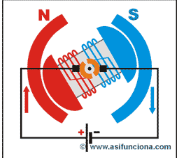
\includegraphics[scale=0.5]{13.png} 
\end{center}

La siguiente figura muestra, de forma animada, el funcionamiento de un motor común bipolar de corriente directa. Como se puede observar, éste consta de un imán permanente en forma de semicírculo, dividido en dos partes fijas al cuerpo del motor. La parte de color rojo del imán corresponde al polo norte “N” y la azul al polo sur “S”. También encontramos un electroimán que a modo de rotor gira entre los polos magnéticos del imán permanente. En el eje del rotor se muestra un colector dividido en dos segmentos y dos escobillas haciendo contacto con los mismos. La batería se encuentra conectada de tal forma que la corriente eléctrica fluye en el sentido convencional con el polo positivo (+) conectado a la escobilla derecha y el polo negativo (–) a la escobilla izquierda. Cada escobilla hace pleno contacto con las secciones del colector, incluso mientras el rotor se encuentra girando.\\

\begin{center}
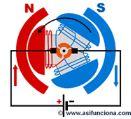
\includegraphics[scale=0.5]{14.png} 
\end{center}
Motor común de corriente directa C.D. con rotor formado por tres polos (rotor tripolar) y colector seccionado en tres partes o segmentos. Este tipo de rotor es el más empleado en los motores de corriente directa de pequeño tamaño.\\
\textbf{MOTORES DE C.D. "SIN ESCOBILLAS" Y "PASO A PASO"}
En algunos equipos de oficina podemos encontrar pequeños motores de C.D. en función de ventiladores para refrescar, por ejemplo, el interior de los ordenadores y otros equipos periféricos. Sin embargo, esos motores poseen características diferentes a los comunes de C.D. ya explicados, pues funcionan “sin escobillas”. Igualmente se fabrican infinidad de juguetes que se mueven empleando motores de ese tipo.\\

\begin{center}
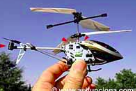
\includegraphics[scale=0.5]{15.png} 
\end{center}

A la izquierda se muestra un motor de C.D. sin escobillas con una hélice acoplada para que funcione como ventilador para refrescar el interior de los ordenadores y otros equipos informáticos. A la derecha vemos un minihelicóptero de juguete controlado por. radio, que también emplea ese mismo tipo de motor. Las puntas de flecha de color rojo señalan la ubicación de los motores que emplea este minihelicóptero para elevarse y permitir dirigir el vuelo por control remoto.\\
Otros equipos de oficina utilizan un tipo de motor de C.D. diferente al común y al de tipo “sin escobillas” y se denomina “paso a paso”. Este otro motor, que funciona también sin escobillas, lo emplean los escáneres para mover la lámpara interna que barre e ilumina las imágenes que deseamos digitalizar, las impresoras láser y de tinta para mover el papel y sus rodillos internos, las grabadoras-lectoras para hacer girar los discos de CDs y DVDs, así como otros dispositivos periféricos para mover sus mecanismos internos.\\

\begin{center}
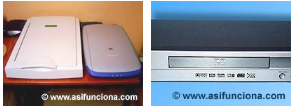
\includegraphics[scale=0.5]{16.png} 
\end{center}
Izquierda: escáneres que emplean motores de C.D. del tipo “paso a paso” para mover la lámpara interna que barre e ilumina las imágenes durante el proceso de digitalización. Derecha: reproductor de discos CDs-DVDs, que emplea también este tipo de motor. \\
La diferencia principal entre los motores comunes de C.D. y los motores “sin escobillas” y “paso a paso” radica en que el electroimán de estos dos últimos se encuentra colocado de forma fija en la carcasa o cuerpo del motor, mientras el imán permanente pasa a ser el rotor.\\



\bibliography{tarea5.bib}{}
\bibliographystyle{http://www.asifunciona.com/electrotecnia/af_motor_cd/af_motor_cd_8.htm\ http://www.mecatronicalatam.com/motores/motores-de-cd}
\end{document}